\section{Implementation Concepts}

\begin{itemize}
\item Files. It is not yet determined how much file level attributes will be 
tracked by the DBS, but this could include size and checksum information.
\end{itemize}

\subsection{Application Parameters}

All general purpose parameters in the DBS are kept in String key/value 
format.  A Parameter Binding entity keeps track of specific key/value pair 
bindings, while a Queryable Parameter Set groups related bindings together. 
(The Parameter Binding table can have duplicates to avoid the overhead of 
an N to N mapping table here, since a key/value pair can obviously belong to 
more than one parameter set.) An Application is described by a single table 
containing application name, version, and edxecutable name.  Finally, the 
mapping table of Application to Parameter Set is the Application 
Configuration.  It is instances of the mapping which are tracked in the 
Processed Dataset.

%\item Application Parameters. The DBS will contain parameters that are deemed 
%interesting for user queries so that the users can find data. The early 
%identified ``important'' parameters such as number of events and estimated 
%luminosity will be stored on table with the Event Collections and Analysis 
%Datasets.  However, we anticipate missing some interesting parameters to 
%start out with, and we also anticipate users wanting to store parameters 
%of interest to specific users for later queries and not general interest 
%parameters.  In the latter cases we envision a generic parameter system that 
%is somewhat slower to query but much more flexible in what it can store. 
%These may include parameters marked as ``queryable'' from the framework, for 
%example.  

\subsection{ Event Collections and Luminosity Estimates}

{\bf FIXME: most of this should be moved elsewhere.}

  There are two points to consider with regards to luminosity.  First of
all, the standard index according to which ``like'' data is aggregated may
be the index of luminosity segments instead of run number.  There may be
several luminosity segments per Event Collection, and summing them may be
the mechanism by which luminosity is assigned to the Event Collections
in the DBS.   Secondly, the DBS should support dataset discovery in
terms of luminosity.  Luminosity should be carried forward through
subsequent processing steps of Event Collections, even in cases of
skims and complicated N to N parentage relationships.  (This is possible
with the existing schema.)  By carrying this information forward, it is
possible to make this part of the API.

Note that this can be combined with buildDataset() to create a luminosity
``snapshot'' within an Analysis Dataset.  In the case alluded to above,
creating a snapshot of an ``open dataset'' is a way of providing a stable
point of reference for analysis when data is being streamed into the
corresponding Data Tier. For example:

\begin{equation}
   /PD/DT/AD = \mbox{buildDataset} ( /PD/DT/DT, AD, \mbox{partialDataset} ( /PD/DT/DT, lumiDesired )[0] )
\end{equation}
could create a ``snapshot'' of interesting that doesn't change as more Event 
Collections are being added to the special $/PD/DT/DT$ Data Tier.


These are shown in figure~\ref{fig:appl}.

\begin{figure}[hbtp]
  \begin{center}
    \resizebox{9cm}{!}{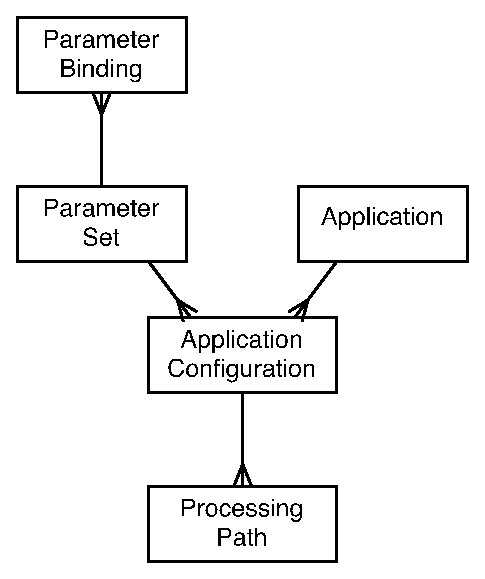
\includegraphics{DatasetBookkeeping-new-2.eps}}
    \caption{Basic outline of the application and parameter tracking parts of the schema. }
    \label{fig:appl}
  \end{center}
\end{figure}

\begin{figure}[hbtp]
  \begin{center}
    \resizebox{9cm}{!}{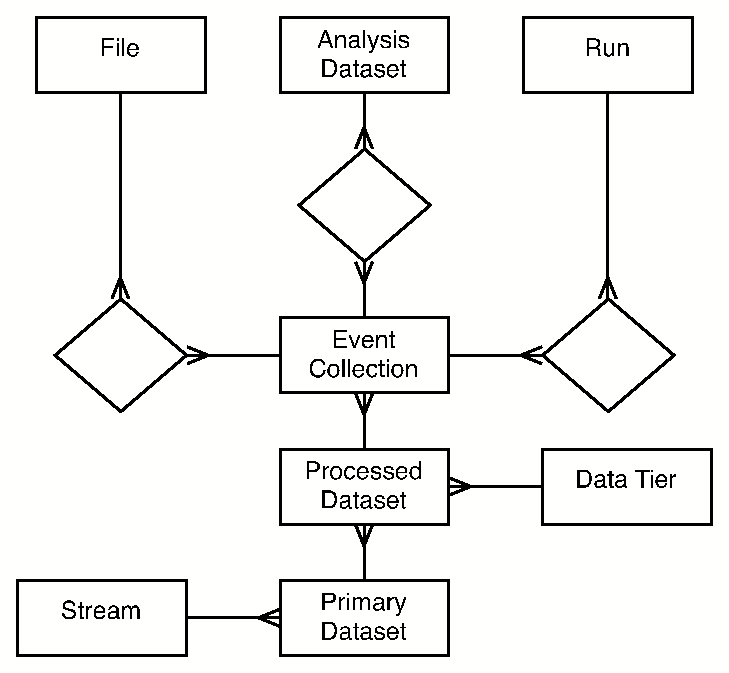
\includegraphics{DatasetBookkeeping-new-1.eps}}
    \caption{Basic outline of the core DBS schema including the basic 
             entities outlined above: Primary Dataset, Processed Dataset, 
             Data Tier, Event Collection, Analysis Dataset, Run, Stream, and 
             File.} 
    \label{fig:highlevel}
  \end{center}
\end{figure}




\begin{figure}[hbtp]
  \begin{center}
    \resizebox{10cm}{!}{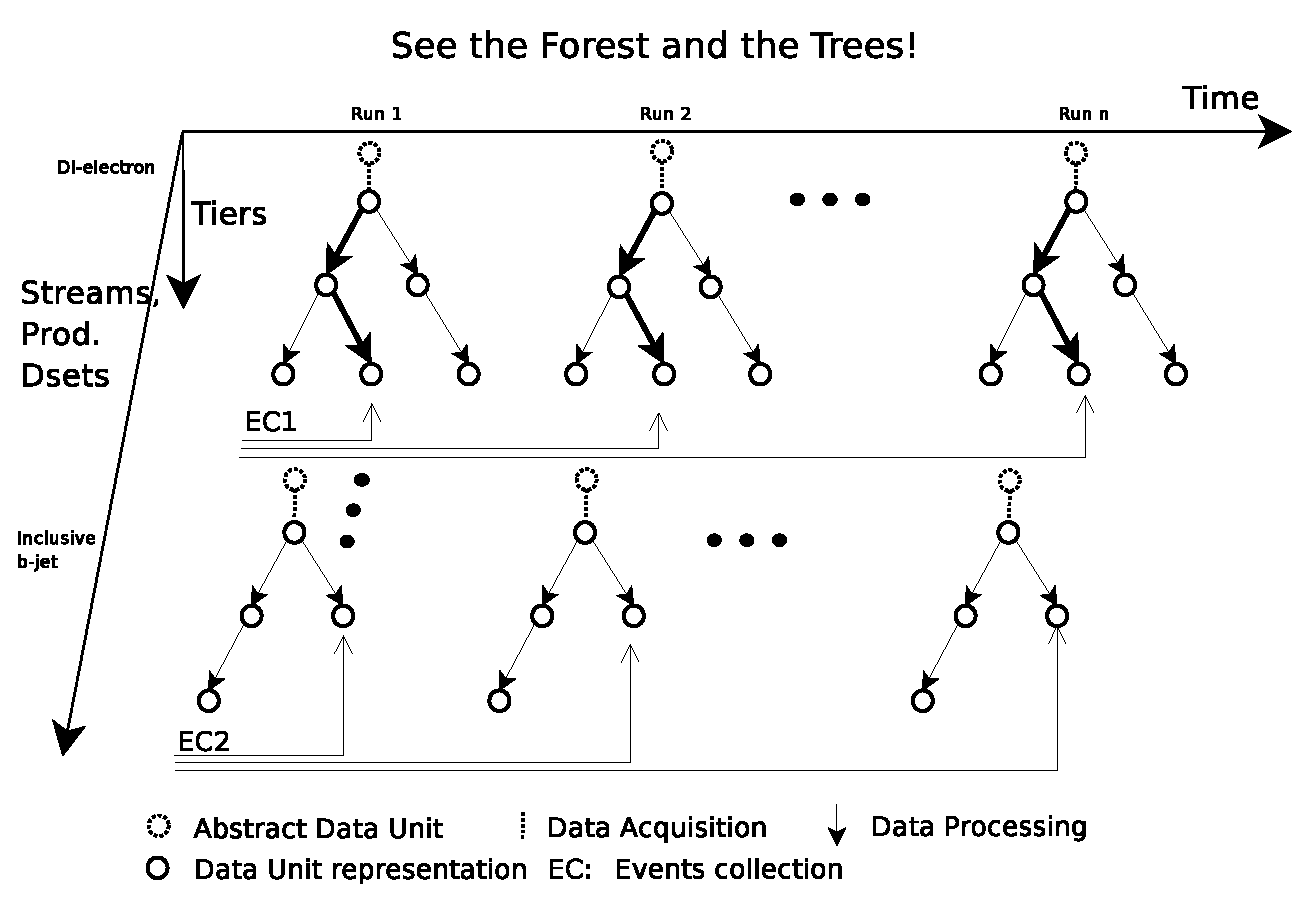
\includegraphics{forest.eps}}
    \caption{The figure shows a forest of trees.  The root of each tree is a 
chunk of data indexed by some number monotonically increasing along the time axis, 
such as run number or luminosity segment.
The path to a node in the tree from the root represents the result of processing 
the root node data through a particular sequence of processing steps.  Each node 
along the way corresponds to an intermediate step.  The individual nodes correspond to objects 
called Event Collections.  Along the axis pointing out of the page, the trees are 
indexed by the qualitative kind of data, or by Primary Dataset. The collection of all 
Event Collections at the same Processing Path within a Primary Dataset is known as a
Processed Dataset. (Exampled of Processed Dataset are unfortunately labeled here 
as ``EC1'' and ``EC2''.)}
    \label{fig:forest}
  \end{center}
\end{figure}


